% ============================================================
% 片段：s04a  对应原文 PDF 第 27--32 页
% 内容：§4 高亏格递推、4.1 $tt^*$ 方程、4.2 $\mathcal{M}$ 的特殊几何、
%       4.3 反常方程及其递推解（含“以费曼图表示的解”小节）
% 译者：t-s04a   审校状态：初稿
% ============================================================

% ==== 原文 PDF 第 27 页 ====

\section{高亏格递推}
\label{sec:4}

\begin{keytakeaways}
  \begin{itemize}[leftmargin=1.4em,itemsep=2pt,topsep=2pt]
    \item \textbf{物理图像}：B 模型本应只被 $(c,c)$ 环的边缘场形变，但来自反环的 $(a,a)$ 形变并不解耦；
          正是这一“解耦失败”使拓扑弦振幅依赖 $\bar z^{\bar\imath}$，从而产生全纯反常，并给出把
          $\mathcal{F}^{(g)}$ 递推联系到较低亏格振幅的方程。
    \item \textbf{数学工具}：用世界面 CPT 算符 $\Theta$ 定义的 $tt^*$ 度规替代拓扑度规，得到形变丛
          $V_{\mathbb{C}}=\mathcal{L}\oplus\mathcal{L}\otimes T\mathcal{M}
          \oplus\overline{\mathcal{L}\otimes T\mathcal{M}}\oplus\overline{\mathcal{L}}$
          上与全纯结构相容的联络 $D_i$、手征环作用矩阵 $C_i$ 与 $C_{\bar\imath}$，以及平坦的
          Gauss--Manin 联络 $\nabla_i=D_i+C_i$。
    \item \textbf{关键结论}：Zamolodchikov 度规 $G_{i\bar\jmath}=g_{i\bar\jmath}/g_{0\bar 0}$ 是凯勒度规，
          $\mathcal{M}$ 是特殊凯勒流形；在 B 模型一侧，$tt^*$ 表述对应 $H^3(X,\mathbb{C})$ 的霍奇分裂的
          非全纯变化，Picard--Fuchs 方程 (4.20) 由 $\nabla$ 的平坦性（矩阵方程 (4.19)）导出。
    \item \textbf{递推结构}：全纯反常方程 (4.24)--(4.26) 把 $\bar\partial_{\bar\imath}\mathcal{F}^{(g)}$
          表示为低亏格振幅与 $\bar C^{jk}_{\bar\imath}$ 的组合；借 $\bar C^{ij}_{\bar\imath}
          =\bar\partial_{\bar\imath}S^{ij}$ 作分部积分，可把解写成以 $S^{ij},S^i,S$ 为传播子的费曼图展开。
  \end{itemize}
\end{keytakeaways}

以下的核心主题是 Bershadsky、Cecotti、Ooguri 与 Vafa（BCOV）的全纯反常方程 \cite{ref18,ref19}。这些方程把
亏格 $g$ 的拓扑弦振幅 $\mathcal{F}^g$（其定义见第（3.2）节）递推地联系到较低亏格的振幅。

BCOV 的推导基于对拓扑弦理论背后的 SCFT 所作的世界面分析。此前的讨论已经表明，视所关注的是哪一个
有限手征环而定，可以从该 SCFT 构造出四种拓扑弦理论。它们分别是与 $(a,c)/(c,a)$ 环及 $(c,c)/(a,a)$ 环
相对应的 A/\emph{anti-A} 模型与 B/\emph{anti-B} 模型。使这些方程的推导得以成立的关键洞见在于：来自
反环（anti-ring）的形变并不解耦。例如，来自 $(a,a)$ 环的形变会对比模型（B-model）的振幅产生影响，
而后者本应只被来自 $(c,c)$ 环的边缘场（marginal field）所形变。分析的出发点是 Cecotti 与 Vafa 的
$tt^*$ 方程 \cite{ref70}。其设置是重新考虑此前讨论过的形变子环，并把一半的态替换为来自世界面 CPT 共轭算符的
态。就霍奇结构的变化而言，两种理论的相互作用导致我们需要考虑霍奇分裂（Hodge split）的非全纯变化，
而不是由 Picard--Fuchs 算符刻画其全纯变化的霍奇滤过（filtration）。由这一变化得到的方程组在超引力的
语言中为人熟知，它们反映矢量多重态标量流形（manifold of the scalars of the vector multiplets）的
特殊几何。概述可参见 \cite{ref51,ref71}。

\subsection{\texorpdfstring{$tt^*$}{tt*} 方程}
\label{sec:4.1}

为陈述 $tt^*$ 方程，把形变丛中的一半态替换为来自世界面 CPT 共轭算符的态。由荷 $(2,2)$ 与 $(3,3)$
的算符所产生、并且此前是相对于拓扑度规以带上标的指标引入的那些态，现改用所谓的 $tt^*$ 度规来替换；
该度规借助世界面 CPT 算符 $\Theta$ 得到\footnote{此处记号沿用 \cite{ref34}。}\footnote{字母表开头的字母取遍
$0,\ldots,n$，而字母表中部的字母只取遍 $1,\ldots,n$。}
\begin{equation}
  g_{a\bar b}=\langle e_a|\Theta e^b\rangle\,.
  \tag{4.1}
  \label{eq:4.1}
\end{equation}

利用该度规，可以如下定义对偶态的一个新基
\begin{equation}
  |e_{\bar\imath}\rangle=g_{k\bar\imath}|e^k\rangle\,,\qquad
  |e_{\bar 0}\rangle=g_{0\bar 0}|e^0\rangle\,.
  \tag{4.2}
  \label{eq:4.2}
\end{equation}

该 $tt^*$ 度规在丛 $\mathcal{V}$ 上诱导出一个与全纯结构相容的联络。它由下式给出
\begin{equation}
  D_i(|e_a\rangle)=\partial_i(|e_a\rangle)-(A_i)^b{}_a(|e_b\rangle)\,,
  \tag{4.3}
  \label{eq:4.3}
\end{equation}

% ==== 原文 PDF 第 28 页 ====

其中 $(A_i)^a{}_b=g^{b\bar c}\partial_i g_{a\bar c}$，而 $(|e_a\rangle)$ 表示向量
$(|e_0\rangle,|e_i\rangle,|e_{\bar\imath}\rangle,|e_{\bar 0}\rangle)^T$；写成矩阵形式，联络为
\begin{equation}
  A_i=
  \begin{pmatrix}
    g^{0\bar 0}\partial_i g_{0\bar 0} & 0 & 0 & 0\\
    0 & g^{l\bar j}\partial_i g_{k\bar j} & 0 & 0\\
    0 & 0 & 0 & 0\\
    0 & 0 & 0 & 0
  \end{pmatrix}\,,\qquad
  A_{\bar\imath}=
  \begin{pmatrix}
    0 & 0 & 0 & 0\\
    0 & 0 & 0 & 0\\
    0 & 0 & g^{l\bar j}\partial_{\bar\imath} g_{k\bar j} & 0\\
    0 & 0 & 0 & g^{0\bar 0}\partial_{\bar\imath} g_{0\bar 0}
  \end{pmatrix}\,.
  \tag{4.4}
  \label{eq:4.4}
\end{equation}

此外，手征环算符 $\phi_i,\phi_{\bar\imath}$ 在此基下的作用成为
\begin{equation}
  \phi_i
  \begin{pmatrix}
    |e_0\rangle\\ |e_j\rangle\\ |e_{\bar\jmath}\rangle\\ |e_{\bar 0}\rangle
  \end{pmatrix}
  =
  \underbrace{
  \begin{pmatrix}
    0 & \delta^k_i & 0 & 0\\
    0 & 0 & C_{ijk}g^{k\bar k} & 0\\
    0 & 0 & 0 & g_{i\bar\jmath}\\
    0 & 0 & 0 & 0
  \end{pmatrix}}_{:=C_i}
  \begin{pmatrix}
    |e_0\rangle\\ |e_k\rangle\\ |e_{\bar k}\rangle\\ |e_{\bar 0}\rangle
  \end{pmatrix}\,,
  \tag{4.5}
  \label{eq:4.5}
\end{equation}
以及
\begin{equation}
  \phi_{\bar\imath}
  \begin{pmatrix}
    |e_0\rangle\\ |e_j\rangle\\ |e_{\bar\jmath}\rangle\\ |e_{\bar 0}\rangle
  \end{pmatrix}
  =
  \underbrace{
  \begin{pmatrix}
    0 & 0 & 0 & 0\\
    g_{\bar\imath j} & 0 & 0 & 0\\
    0 & C_{\bar\imath\bar\jmath\bar k}g^{\bar k k} & 0 & 0\\
    0 & 0 & \delta^{\bar k}_{\bar\imath} & 0
  \end{pmatrix}}_{:=C_{\bar\imath}}
  \begin{pmatrix}
    |e_0\rangle\\ |e_k\rangle\\ |e_{\bar k}\rangle\\ |e_{\bar 0}\rangle
  \end{pmatrix}\,.
  \tag{4.6}
  \label{eq:4.6}
\end{equation}

% [Tutor Note: 易错点] (4.4)--(4.6) 的块位置、零结构与矩阵乘法的哑指标读法
\begin{yizhu}[易错点]
(4.4) 中 $A_i$ 只有两个非零元（第 1 行第 1 列与第 2 行第 2 列），$A_{\bar\imath}$ 的非零元则在第 3 行
第 3 列与第 4 行第 4 列；中间块的指标约定是 $(A_i)^k{}_l=g^{l\bar j}\partial_i g_{k\bar j}$（上标 $l$
为列、下标 $k$ 为行），与 $(A_i)^a{}_b=g^{b\bar c}\partial_i g_{a\bar c}$ 中 $a=k,b=l$ 一致，抄写时
勿写成 $g^{k\bar j}\partial_i g_{l\bar j}$，也不要对调 $A_i$、$A_{\bar\imath}$ 的块位置。
(4.5)--(4.6) 两端的列向量是同一个态向量的两种哑指标写法：左端标
$(|e_0\rangle,|e_j\rangle,|e_{\bar\jmath}\rangle,|e_{\bar 0}\rangle)$，右端标
$(|e_0\rangle,|e_k\rangle,|e_{\bar k}\rangle,|e_{\bar 0}\rangle)$，矩阵按“行乘列”作用。按此读法，
(4.5) 第 1 行给出 $\phi_i|e_0\rangle=\delta^k_i|e_k\rangle=|e_i\rangle$，(4.6) 第 4 行给出
$\phi_{\bar\imath}|e_{\bar 0}\rangle=\delta^{\bar k}_{\bar\imath}|e_{\bar k}\rangle=|e_{\bar\imath}\rangle$，
中间各行则分别给出 $C_{ij}{}^{\bar k}=C_{ijk}g^{k\bar k}$、$g_{i\bar\jmath}$、
$g_{\bar\imath j}$、$C_{\bar\imath\bar\jmath}{}^{k}=C_{\bar\imath\bar\jmath\bar k}g^{\bar k k}$ 的耦合；
若把两端的态标签误当作矩阵的行指标去逐项比较，会以为原文的上下标自相矛盾。
\end{yizhu}

正如前面所指出的，SCFT 的基态 $|e_0\rangle$ 在相差一个标度的意义下是唯一的。这意味着它是模空间
$\mathcal{M}$ 上某个线丛 $\mathcal{L}$ 的一个截面。此外，由于 $|e_i\rangle$ 这些态是由同时参数化理论
形变的算符所产生，它们可以与 $\mathcal{L}\otimes T\mathcal{M}$ 的截面等同起来。它们之所以也是该线丛的
截面，是因为它们从基态继承了任意的标度。于是，基态的丛可以组织为
\begin{equation}
  V_{\mathbb{C}}=\mathcal{L}\oplus\mathcal{L}\otimes T\mathcal{M}
  \oplus\overline{\mathcal{L}\otimes T\mathcal{M}}\oplus\overline{\mathcal{L}}\,.
  \tag{4.7}
  \label{eq:4.7}
\end{equation}

现在可以具体写出 $tt^*$ 方程 \cite{ref70}\footnote{教学性的推导见 \cite{ref9}。}
\begin{equation}
  \begin{aligned}
    [D_i,D_j]&=0\,, & [D_{\bar\imath},D_{\bar\jmath}]&=0\,,\\
    [D_i,C_j]&=[D_j,C_i]\,, & [D_{\bar\imath},C_{\bar\jmath}]&=[C_{\bar\imath},D_{\bar\jmath}]\,,\\
    [D_i,D_{\bar\imath}]&=-[C_i,C_{\bar\imath}]\,.
  \end{aligned}
  \tag{4.8}
  \label{eq:4.8}
\end{equation}

其中最后一个方程特别有意思，因为它允许定义一个曲率为零的修正联络
\begin{equation}
  \nabla_i=D_i+C_i\,,\qquad
  \nabla_{\bar\imath}=D_{\bar\imath}+C_{\bar\imath}\,,\qquad
  [\nabla_i,\nabla_{\bar\imath}]=0\,.
  \tag{4.9}
  \label{eq:4.9}
\end{equation}

% [Tutor Note: 物理图像] $tt^*$ 度规与手征环插入的物理含义，Gauss--Manin 联络的平坦性
\begin{yizhu}[物理图像]
$tt^*$ 方程的核心是“把求导换成插入”：在特殊坐标 $t^i$ 下，沿 $i$ 方向的形变由边缘算符 $\phi_i$ 的
插入实现，故 $\partial_{t^i}$ 对应于插入 $\phi_i$；但在一般坐标 $z^i$ 下，基向量 $|e_a\rangle$ 随模参数
转动，求导必须先扣除这一转动，于是出现联络 $A_i$（(4.3)）。手征环算符的作用矩阵 $C_i$（(4.5)）是
“插入本身”的矩阵元，$D_i$ 是“扣除基转动”后的协变导数，二者的和 $\nabla_i=D_i+C_i$（(4.9)）把两步合并，
因而是 Gauss--Manin 联络；其平坦性 $[\nabla_i,\nabla_{\bar\imath}]=0$ 正是 Picard--Fuchs 方程 (4.20)
的来源。另一方面，用世界面 CPT 算符 $\Theta$ 定义的 $tt^*$ 度规 (4.1) 取代拓扑度规，等价于把形变丛的
一半指标换成 CPT 共轭态，从而使霍奇滤过（全纯变化）升级为霍奇分裂（非全纯变化），(4.12) 即这一对应。
\end{yizhu}

这个联络就是 Gauss--Manin 联络，在前面对拓扑场论与霍奇结构变化的讨论中已经遇到过。

% ==== 原文 PDF 第 29 页 ====

\subsection{\texorpdfstring{$\mathcal{M}$}{M} 的特殊几何}
\label{sec:4.2}

$V_{\mathbb{C}}$ 上的 $tt^*$ 度规还可以通过在 $T\mathcal{M}$ 取值部分及其复共轭上的限制，用来在
$\mathcal{M}$ 上定义一个度规。以此方式得到的度规就是 Zamolodchikov 度规，其定义为
\begin{equation}
  G_{i\bar\jmath}=\frac{g_{i\bar\jmath}}{g_{0\bar 0}}\,.
  \tag{4.10}
  \label{eq:4.10}
\end{equation}
进一步令
\[
  g_{0\bar 0}:=e^{-K}\,,
\]
则可证明 $G_{i\bar\jmath}=\partial_i\partial_{\bar\jmath}K$，因而 Zamolodchikov 度规是凯勒的。此外，
(4.8) 的最后一个方程可以翻译为关于 $G_{i\bar\jmath}$ 曲率的如下陈述
\begin{equation}
  R_{i\bar\imath}{}^{l}{}_{j}=[\bar\partial_{\bar\imath},D_i]^l{}_j
  =\bar\partial_{\bar\imath}\Gamma^l_{ij}
  =\delta^l_iG_{j\bar\imath}+\delta^l_jG_{i\bar\imath}-C_{ijk}C^{kl}_{\bar\imath}\,,
  \tag{4.11}
  \label{eq:4.11}
\end{equation}
% [原文疑误: (4.11) 末项 C^{kl}_{\bar\imath} 疑漏上划线，应为 \bar C^{kl}_{\bar\imath}：R 含 \bar\partial_{\bar\imath} 导数，该项须反全纯；对照下文 \bar C^{jk}_{\bar\imath} 的定义与 (4.25)。照抄原文。]
其中 $D$ 是协变导数，其联络部分（视所作用的丛而定）由上下文给出
\[
  \Gamma^k_{ij}=G^{k\bar k}\partial_i G_{\bar kj}\,,\qquad\text{以及}\qquad K_i=\partial_iK\,,
\]
分别对应于余切丛与线丛，并且
\[
  \bar C^{jk}_{\bar\imath}:=e^{2K}G^{k\bar k}G^{l\bar l}\bar C_{\bar\imath\bar k\bar l}\,.
\]
% [原文疑误: 左端自由指标 j,k,\bar\imath 与右端自由指标 k,l,\bar\imath 不匹配（j、l 均未配对）；按 (4.25) 的约定与 (4.11) 末项的用法，右端应为 e^{2K}G^{j\bar k}G^{k\bar l}\bar C_{\bar\imath\bar k\bar l}（等价地，左端可写作 \bar C^{kl}_{\bar\imath}）。照抄原文。]

% [Tutor Note: 原文疑误] (4.11) 及 p31 (4.26) 缺上划线、p29 定义的指标不匹配
\begin{yizhu}[原文疑误]
原文写作 $\bar C^{jk}_{\bar\imath}:=e^{2K}G^{k\bar k}G^{l\bar l}\bar C_{\bar\imath\bar k\bar l}$：左端的
自由指标是 $j,k,\bar\imath$，右端的自由指标却是 $k,l,\bar\imath$，$j$ 与 $l$ 均未配对。按 (4.25) 的
指标约定 $\bar C^{ij}_{\bar k}=\bar C_{\bar\imath\bar\jmath\bar k}G^{i\bar\imath}G^{j\bar\jmath}e^{2K}$，
右端应为 $e^{2K}G^{j\bar k}G^{k\bar l}\bar C_{\bar\imath\bar k\bar l}$（等价地，左端可写作
$\bar C^{kl}_{\bar\imath}$）。此外，(4.11) 与 (4.26) 中的 $C^{kl}_{\bar\imath}$ 疑漏上划线，应为
$\bar C^{kl}_{\bar\imath}$：因为 $R_{i\bar\imath}{}^l{}_j$ 含 $\bar\partial_{\bar\imath}$ 导数，该项须
反全纯，且前文所定义者正是 $\bar C$。以上各处均照原文转写，未作改动。
\end{yizhu}

凯勒条件连同曲率条件使流形 $\mathcal{M}$ 成为特殊凯勒流形，其几何称为特殊几何。（见
\cite{ref56,ref51,ref71,ref59} 及其中的参考文献。）在此设置下，汤川耦合是 $\mathcal{L}^2\otimes\mathrm{Sym}^3T^*
\mathcal{M}$ 的一个全纯截面。

下面将说明，形变丛几何的 $tt^*$ 表述在 B 模型一侧对应于霍奇丛的非全纯变化
\begin{equation}
  V_{\mathbb{C}}=H^3(X,\mathbb{C})=H^{3,0}(X)\oplus H^{2,1}(X)\oplus H^{1,2}(X)
  \oplus H^{0,3}(X)\,.
  \tag{4.12}
  \label{eq:4.12}
\end{equation}
取 $\mathcal{L}$ 的截面为相差一个标度唯一的全纯 $(3,0)$ 形式 $\Omega\in H^{3,0}(X)$，并用形式的外积
（wedge product）在 $X$ 上积分给出内积，则线丛上的度规为
\begin{equation}
  g_{0\bar 0}=e^{-K}=-i\int_X\Omega\wedge\bar\Omega\,.
  \tag{4.13}
  \label{eq:4.13}
\end{equation}
可以如下定义 $H^{2,1}$ 与 $H^{1,2}$ 中的元素
\begin{equation}
  \chi_i:=D_i\Omega=(\partial_i+K_i)\Omega\,,\qquad
  \bar\chi_{\bar\imath}:=D_{\bar\imath}\bar\Omega
  =(\partial_{\bar\imath}+K_{\bar\imath})\bar\Omega\,.
  \tag{4.14}
  \label{eq:4.14}
\end{equation}
其内积为
\begin{equation}
  g_{i\bar\jmath}=i\int_X\chi_i\wedge\bar\chi_{\bar\jmath}
  =e^{-K}G_{i\bar\jmath}=e^{-K}\partial_i\partial_{\bar\jmath}K\,.
  \tag{4.15}
  \label{eq:4.15}
\end{equation}

% ==== 原文 PDF 第 30 页 ====

定义汤川耦合
\begin{equation}
  C_{ijk}:=-\int_X\Omega\wedge D_iD_jD_k\Omega
  =-\int_X\Omega\wedge\partial_i\partial_j\partial_k\Omega\,,
  \tag{4.16}
  \label{eq:4.16}
\end{equation}
可以算出
\begin{equation}
  D_iD_j\Omega=D_i\chi_j=iC_{ijk}e^K G^{k\bar k}\bar\chi_{\bar k}\,,\qquad
  D_i\bar\chi_{\bar\imath}=G_{i\bar\imath}\bar\Omega\,.
  \tag{4.17}
  \label{eq:4.17}
\end{equation}
取 $V_{\mathbb{C}}$ 的如下截面向量
\begin{equation}
  \vec{\Omega}=(\Omega,\chi_i,\bar\chi_{\bar\imath},\bar\Omega)\,,
  \tag{4.18}
  \label{eq:4.18}
\end{equation}
即可得到 Gauss--Manin 联络
\begin{equation}
  D_i
  \begin{pmatrix}
    \Omega\\ \chi_j\\ \bar\chi_{\bar\jmath}\\ \bar\Omega
  \end{pmatrix}
  =
  \begin{pmatrix}
    0 & \delta^k_i & 0 & 0\\
    0 & 0 & iC_{ijk}e^K G^{k\bar k} & 0\\
    0 & 0 & 0 & G_{i\bar\jmath}\\
    0 & 0 & 0 & 0
  \end{pmatrix}
  \begin{pmatrix}
    \Omega\\ \chi_k\\ \bar\chi_{\bar k}\\ \bar\Omega
  \end{pmatrix}\,.
  \tag{4.19}
  \label{eq:4.19}
\end{equation}
这一矩阵方程可以翻译为关于 $\Omega$ 的如下四阶微分方程
\begin{equation}
  D_mD_n(C_i^{-1})^{lj}D_iD_j\Omega=0\,,
  \tag{4.20}
  \label{eq:4.20}
\end{equation}
它就是 Picard--Fuchs 方程。文献 \cite{ref58,ref51} 表明，该方程等价于此前遇到的全纯 Picard--Fuchs 方程，
并且选取霍奇结构的非全纯变化不过是向量 $\vec{\Omega}$ 的一个规范选择。

\subsection{反常方程及其递推解}
\label{sec:4.3}

前文已论证，拓扑弦理论的形变对应于在作用量 $S$ 中加入如下形式的项
\[
  z^i\int\phi_i^{(2)}+\bar z^{\bar\imath}\int\bar\phi_{\bar\imath}^{(2)}\,,
\]
$z^i$ 是 $\mathcal{M}$ 上的复坐标；记号从 $t^i$ 改为 $z^i$，是为了显式区分拓扑／特殊坐标 $t^i$ 与更
一般的坐标 $z^i$：对前者求导对应于插入，而对后者作插入则对应于取协变导数。因此，带有 $n$ 个
边缘 $(c,c)$ 场后代（descendant）插入的振幅（对 B 模型而言）可由下式定义 \cite{ref19}
\begin{equation}
  \mathcal{F}^{(g)}_{i_1\ldots i_n}=D_{i_n}\mathcal{F}^{(g)}_{i_1\ldots i_{n-1}}\,.
  \tag{4.21}
  \label{eq:4.21}
\end{equation}
另一方面，对 $\bar z^{\bar\imath}$ 求导对应于插入一个边缘 $(a,a)$ 算符的后代
\begin{equation}
  \phi_{\bar\imath}^{(2)}=dzd\bar z\{G^+,[\bar G^+,\phi_{\bar\imath}]\}
  =-\frac12 dzd\bar z\{G^++\bar G^+,[G^+-\bar G^+,\phi_{\bar\imath}]\}\,.
  \tag{4.22}
  \label{eq:4.22}
\end{equation}

% ==== 原文 PDF 第 31 页 ====

在拓扑\emph{场}论中，这样的插入在关联函数中会消失，因为该方程的第二部分表明该算符是 $Q_B$-恰当的。
场论中关于这种解耦的论证是：$Q_B$ 是理论的对称性，可以让它穿过关联函数，直到它作用在基态上并给出零。
在拓扑弦理论的情形，这一论证失效；下面概述其原因。$\mathcal{F}^g$ 的公式再次给出为
\begin{equation}
  \mathcal{F}^g=\int_{\mathcal{M}_g}[dm\,d\bar m]
  \Big\langle\prod_{a=1}^{3g-3}\Big(\int_\Sigma\mu_aG^-\Big)
  \Big(\int_\Sigma\bar\mu_a\bar G^-\Big)\Big\rangle_{\Sigma_g}\,,
  \tag{4.23}
  \label{eq:4.23}
\end{equation}

% [Tutor Note: 物理图像] 反常来自黎曼面模空间的边界（节点退化）
\begin{yizhu}[物理图像]
反常的物理来源是黎曼面模空间 $\mathcal{M}_g$ 的边界。(4.23) 把 $\mathcal{F}^g$ 写成 $\mathcal{M}_g$ 上
的积分；把 $G^+$（或 $\bar G^+$）穿过关联函数时，它命中与 Beltrami 微分缩并的 $G^-$（或 $\bar G^-$），
由超共形代数给出能动张量 $T$。$T$ 度量理论对世界面度规变分的响应，故等价于
$\partial^2/\partial m\partial\bar m$；于是对 $\mathcal{M}_g$ 的全导数积分只剩边界项。$\mathcal{M}_g$ 的
边界正是黎曼面退化为节点的构型：要么分裂为亏格 $g_1$ 与 $g_2=g-g_1$ 的两部分，要么从亏格 $g-1$ 的面上
长出一支环柄（见后图的两类图形）。这些边界构型上的 $G^\pm$ 缩并贡献出
$\bar C^{jk}_{\bar\imath}D_j\mathcal{F}D_k\mathcal{F}$ 与 $\bar C^{jk}_{\bar\imath}D_jD_k
\mathcal{F}^{(g-1)}$ 两类项，即 (4.24)；完整推导见 \cite{ref18,ref19}。
\end{yizhu}

可以看出，在把 $G^+$ 与 $\bar G^+$ 穿过定义 $\mathcal{F}^g$ 的关联函数时，它们会命中与 Beltrami 微分
缩并的 $G^-$ 与 $\bar G^-$，由超共形代数这给出能动张量 $T$。能动张量反过来度量理论对度规变分的响应，
因而可以换成黎曼面模空间 $\mathcal{M}_g$ 上的导数 $\frac{\partial^2}{\partial m\partial\bar m}$，因为
后者恰好参数化这类改变。于是最终只剩下黎曼面模空间上关于黎曼面模的导数的积分，它在差一个边界贡献的
意义下为零。正是这些来自黎曼面模空间边界的贡献被整理进全纯反常方程。下图以图解方式描绘了这些贡献；
方程的完整推导请参阅原始文献 \cite{ref18,ref19}。方程如下
\begin{equation}
  \bar\partial_{\bar\imath}\mathcal{F}^{(g)}=\frac12\bar C^{jk}_{\bar\imath}
  \Big(\sum_{g_1+g_2=g}D_j\mathcal{F}^{(g_1)}D_k\mathcal{F}^{(g_2)}
  +D_jD_k\mathcal{F}^{(g-1)}\Big)\,,
  \tag{4.24}
  \label{eq:4.24}
\end{equation}

\begin{figure}[htbp]
  \centering
  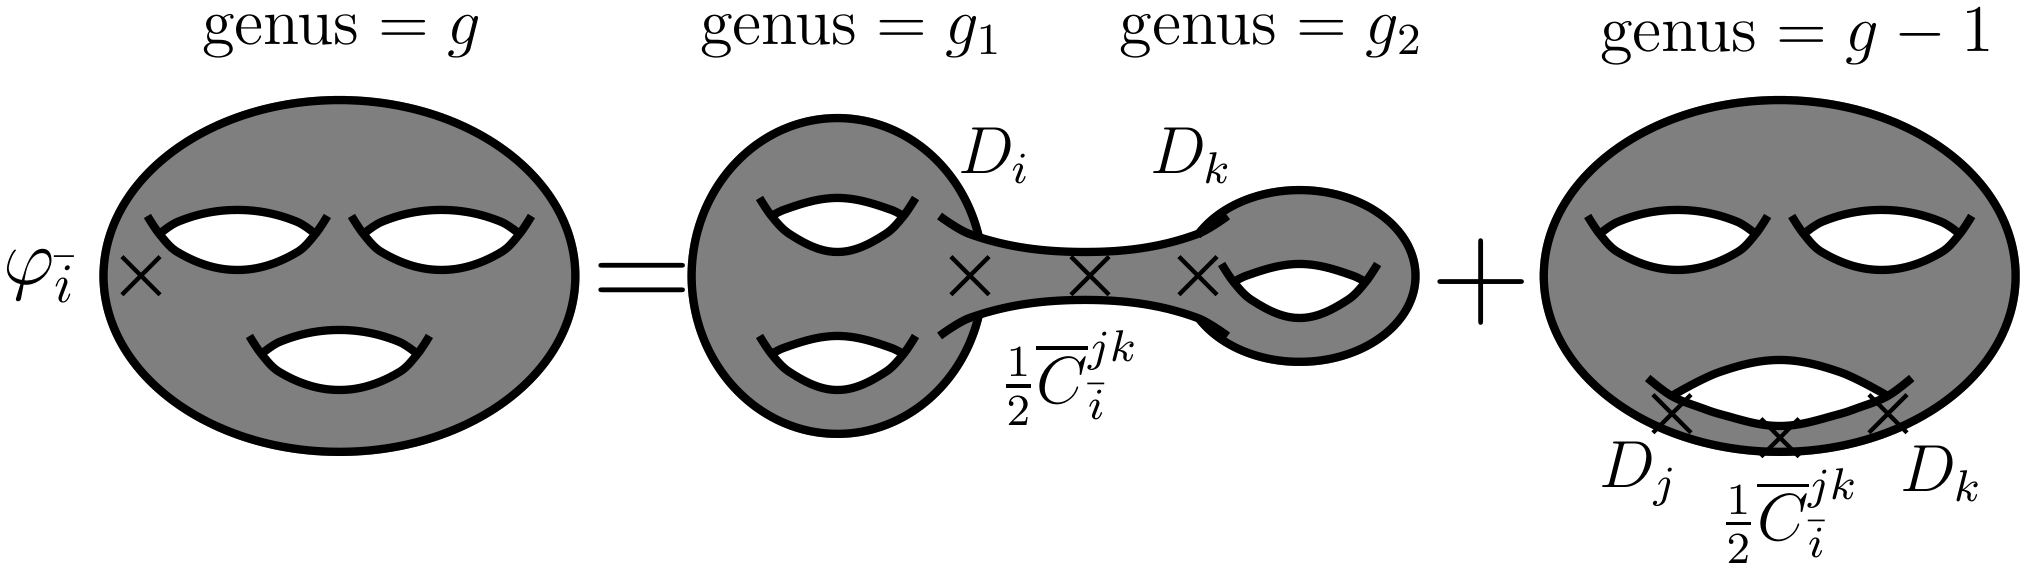
\includegraphics[width=0.95\linewidth]{figures/figure-1.png}
  \caption{全纯反常方程 (4.24) 的费曼图式图解：左侧为亏格 $g$ 的黎曼面，其上有算符
    $\phi_{\bar\imath}$ 的插入（以 $\times$ 标记）；右端为两类退化情形——中间是亏格 $g_1$ 与 $g_2$
    （$g_1+g_2=g$）的两部分经由一条细管相连，最右是亏格 $g-1$ 的黎曼面；$D_i,D_j,D_k$ 表示对相应
    模参数的协变导数，$\frac12\bar C^{jk}_{\bar\imath}$ 为相应的耦合因子。（原文第 31 页，式 (4.24)
    之后；原文未编号，此处编号为译者所加）}
  \label{fig:1}
\end{figure}

其中 $g>1$，并且
\begin{equation}
  \bar C^{ij}_{\bar k}=\bar C_{\bar\imath\bar\jmath\bar k}G^{i\bar\imath}G^{j\bar\jmath}e^{2K}\,,\qquad
  \bar C_{\bar\imath\bar\jmath\bar k}=\overline{C_{ijk}}\,.
  \tag{4.25}
  \label{eq:4.25}
\end{equation}
对 $g=1$，方程为
\begin{equation}
  \bar\partial_{\bar\imath}\mathcal{F}^{(1)}_j
  =\frac12C_{jkl}C^{kl}_{\bar\imath}
  +\Big(1-\frac{\chi}{24}\Big)G_{j\bar\imath}\,.
  \tag{4.26}
  \label{eq:4.26}
\end{equation}
% [原文疑误: 同 (4.11)，此处 C^{kl}_{\bar\imath} 疑漏上划线，应为 \bar C^{kl}_{\bar\imath}。照抄原文。]

% [Tutor Note: 易错点] 反常方程的归一化因子、$1/2$ 与有序求和、$\chi/24$ 修正、指标升降
\begin{yizhu}[易错点]
此处最易出错的是因子与求和约定：(i) (4.24) 的 $\frac12$ 与 $\sum_{g_1+g_2=g}$ 配套——求和遍历
有序对 $(g_1,g_2)$，故 $1/2$ 不可漏；第二项 $D_jD_k\mathcal{F}^{(g-1)}$ 不属于该求和。(ii) $g=1$ 时
(4.24) 的求和退化，须改用 (4.26)，其中 $\chi$ 是 Calabi--Yau 三维流形的 Euler 数，$(1-\chi/24)$ 是
$g=1$（单圈）反常方程的已知系数；$\frac12C_{jkl}C^{kl}_{\bar\imath}$ 的两个上标 $k,l$ 与 $C_{jkl}$
完全缩并，漏一个因子便破坏 $\bar\partial_{\bar\imath}\mathcal{F}^{(1)}_j$ 的 $(1,1)$ 型。
(iii) 指标升降要用 Zamolodchikov 度规的逆 $G^{i\bar\imath}$ 而非原度规 $g^{i\bar\imath}$：由
$g_{0\bar 0}=e^{-K}$ 与 (4.15) 得 $g^{i\bar\jmath}=e^{K}G^{i\bar\jmath}$；而 (4.25) 中的 $e^{2K}$ 是为
补足 $\bar C$ 的线丛权，不可与逆度规的 $e^{K}$ 因子混为一谈。(4.13) 的 $-i$ 与 (4.15) 的 $+i$ 也不可
互换。
\end{yizhu}

% ==== 原文 PDF 第 32 页 ====

\subsubsection*{以费曼图表示的解}

BCOV 在提出反常方程 \cite{ref19} 的同时，也提出了递推求解 $\mathcal{F}^{(g)}$ 的方法。其想法是对反常方程中
出现的反全纯导数作分部积分，直到得到如下形式的表达式
\[
  \partial_{\bar\imath}A=\partial_{\bar\imath}B\ \Rightarrow\ A=B+f(z)\,,
\]
其中 $f(z)$ 是全纯模糊性（holomorphic ambiguity）。为了在实践中做到这一点，他们首先注意到反全纯汤川
耦合可以局部地写为
\[
  \bar C_{\bar\imath\bar\jmath\bar k}=e^{-2K}D_iD_j\bar\partial_{\bar k}S\,,
\]
其中 $S$ 是 $\mathcal{L}^{-2}$ 的截面。还可以进一步引入一些对象 $S^{ij}$、$S^i$，它们分别是
$\mathcal{L}^{-2}\otimes\mathrm{Sym}^2(T^*\mathcal{M})$ 与 $\mathcal{L}^{-2}\otimes
T^*(\mathcal{M})$ 的截面，使得
\begin{equation}
  \bar\partial_{\bar\imath}S^{ij}=\bar C^{ij}_{\bar\imath}\,,\qquad
  \bar\partial_{\bar\imath}S^j=G_{i\bar\imath}S^{ij}\,,\qquad
  \bar\partial_{\bar\imath}S=G_{i\bar\imath}S^i\,.
  \tag{4.27}
  \label{eq:4.27}
\end{equation}
现在的做法是依次对反常方程作分部积分，首先写出
\begin{equation}
  \begin{aligned}
    &\bar\partial_{\bar\imath}\Big(\mathcal{F}^{(g)}
      -\frac12S^{jk}\Big(\sum_{g_1+g_2=g}D_j\mathcal{F}^{(g_1)}D_k\mathcal{F}^{(g_2)}
      +D_jD_k\mathcal{F}^{(g-1)}\Big)\Big)\\
    &\qquad=-\frac12S^{jk}\bar\partial_{\bar\imath}
      \Big(\sum_{g_1+g_2=g}D_j\mathcal{F}^{(g_1)}D_k\mathcal{F}^{(g_2)}
      +D_jD_k\mathcal{F}^{(g-1)}\Big)\,,
  \end{aligned}
  \tag{4.28}
  \label{eq:4.28}
\end{equation}
然后反复使用所得到的曲率表达式 $[\bar\partial_{\bar\imath},D_j]$（即 (4.11)）以及 $\tilde g<g$ 时
$\bar\partial_{\bar\imath}\mathcal{F}^{\tilde g}$ 的已知结果，即可得到所需结论。他们进一步指出，
如果把该系统视为比模空间 $\mathcal{M}$ 的维数多一个自由度的量子系统，则由此得到的表达式类似于费曼图：
其传播子为
\[
  K^{ij}=-S^{ij}\,,\qquad K^{i\phi}=-S^i\,,\qquad\text{以及}\qquad K^{\phi\phi}=-2S\,,
\]
而顶点由带插入的关联函数给出。此外，他们还给出了按费曼图展开的证明。

% [Tutor Note: 物理图像] 分部积分与费曼图递推的组合结构、全纯模糊性的地位
\begin{yizhu}[物理图像]
(4.28) 的关键是用 $\bar\partial_{\bar\imath}S^{ij}=\bar C^{ij}_{\bar\imath}$（(4.27)）把反常方程改写成
“左端只含 $\bar\partial_{\bar\imath}\mathcal{F}^{(g)}$ 与非全纯汤川耦合、右端只含较低亏格振幅的
$\bar\partial_{\bar\imath}$”的形式；反复使用 (4.11) 给出的 $[\bar\partial_{\bar\imath},D_j]$ 与已知的
$\bar\partial_{\bar\imath}\mathcal{F}^{\tilde g}$（$\tilde g<g$）即可逐级积分出 $\mathcal{F}^{(g)}$。
把 $S^{ij},S^i,S$ 视为传播子、把汤川耦合与带插入的关联函数视为顶点，则每一次分部积分相当于在图上接
一条内线或一个顶点，而图的亏格就是所计算的亏格——这正是“以费曼图表示的解”的含义；原文提到该系统比
$\mathcal{M}$ 多一个自由度，对应的就是 $S$ 那条带 $\phi$ 指标的传播子链。需注意递推只确定非全纯部分，
全纯模糊性 $f(z)$ 必须在每一步由边界条件固定（原文此处未展开，见 \cite{ref19} 及后文）。
\end{yizhu}

然而，这一做法的一个实际缺点是迭代次数增长极快，$\mathcal{F}^{(g)}$ 的表达会变得很长。另一方面，
反常方程所包含的递推信息在每一步都需要用边界条件来补充，以确定全纯模糊性。
